\appendix 
\thispagestyle{empty}

\hypertarget{AppendixA}{}\section*{Appendix A: The Road Side Unit (RSU)} \label{sec:RSU}
According to \cite{kherroubi2020novel}, the RSU architecture is composed of two main modules, the perception module and the communication module. 
        \begin{figure}[!h]
        \centering 
        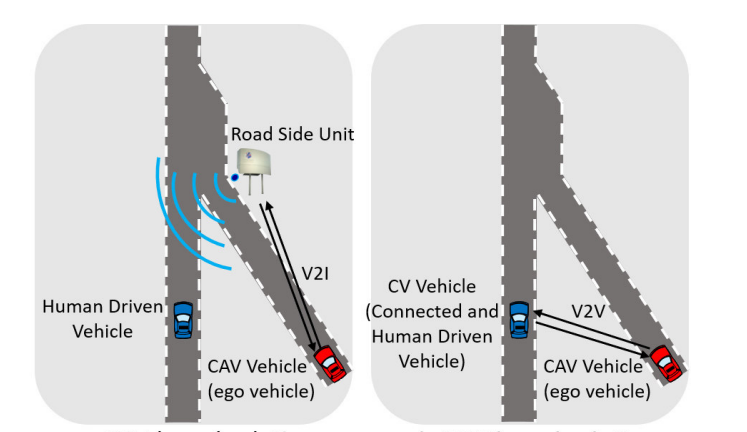
\includegraphics[width=11cm,height=18cm,keepaspectratio]{chapters/Chapitre_4/Figures/RSU}
        \vspace{-2.3mm}
        \caption{Road Side Unit (RSU)}
        \label{fig:RSU}
        \vspace{-5mm}
        \end{figure}


\begin{itemize}
    \item \textbf{(a) The RSU perception module:} It is equipped with an array of sensors such as cameras, RADAR, and LiDAR. The RSU significantly extends the range and reliability of perception compared to relying solely on the on-board sensors of the individual vehicles. This augmentation of perception capabilities plays a pivotal role in enhancing the overall safety and efficiency of the MVS. 

    For instance, in \cite{chen2019architecture}, the authors introduced a novel application of the RSU involving a 360-degree LiDAR, transforming the RSU into a LiDAR-enhanced infrastructure. Similarly, in \cite{masi2021augmented}, a collaborative map-aided tracking system was proposed, combining an on-board LiDAR sensor and a road side vision system. This fusion of sensor data allowed for the broadcasting of detected objects, contributing to an improved situation awareness. Moreover, the work in \cite{geissler2018designing}, viewed the sensor infrastructure as a valuable tool for supporting various vehicles activities. This could involve enhancing agent-based vision systems or optimizing traffic management through more established motion coordination. 





  \item \textbf{(b) The RSU communication module:} It utilizes stationary perception sensors that gather object detection and tracking data, and through a data fusion process, it derives detailed object characteristics such as position, heading, and speed for each detected object. This capability allows the RSU to provide rich and comprehensive information about the detected object. 

  Additionally, the RSU employs the V2X communication technologies as discussed in section \ref{sec:communication_module} to broadcast the objects data as in Figure \ref{fig:RSU}. Presently, V2X systems predominantly rely on two technologies: Dedicated Short-Range Communications (DSRC) and cellular-based V2X technology. These communication mechanisms enable the RSU to exchange critical information with nearby vehicle (cf. Figure \ref{fig:RSU}); within the communication range of the communication devices, facilitating enhanced situational awareness and coordination with the MVS. 
\end{itemize}


%% ---------------------------------- Fin de la partie sur les RSU -----------------------

